\documentclass{article}
\usepackage{float}
\usepackage{graphicx} %package to manage images
\usepackage[utf8]{inputenc}
\usepackage[a4paper, total={6in, 8in}]{geometry}
\usepackage{xurl}
\title{Relatório 3 \\ Ajuste das análises}
\author{Pedro A. S. O. Neto}
\date{Fevereiro 2022}

\begin{document}

\maketitle

\section{Tarefas executadas}

O código foi alterado para atender às observações do Victor, feitas no email de $11.02.2022$. Agora os gráficos parecem estar consistentes com os vídeos. 

\section{Problemas}

\subsection{Problema 1}
Alguns tempos de fixação são bem pequenos (e.g., 8ms) e não aparecem nos vídeos, nem nos gráficos que eu estou fazendo. Por exemplo, considere a tabela e o gráfico no final do documento. A participante Dovalys, trial IJA.A1.B1.E, teve algumas fixações de 8ms, que não aparecem no gráfico e nem nos vídeos da tarefa.

\subsection{Problema 2}
Sobre a questão das ficações de $8ms$, eu posso agrupá-las e somar todas as fixações que aparecem em sequência como uma grande ficação, como o Victor sugeriu. Mas isso vem com alguns problemas. 


O algorítmo do TOBII faz um agrupamento automático de fixações próximas (tanto em tempo quanto em local). No entanto, se nós limitarmos as fixações a uma duração de $8ms$, o programa é obrigado a interpretar todo pequeno desvio da AOI como uma nova fixação. Um exemplo disso é a trial RJA.A1.B2.D, da participante Abacaxi (Figura 3).

Um outro problema do Gaze.event.duration é que não existe, em nenhum dos dados que eu recebi, nenhuma fixação diferente de 8ms. Eu imagino que, no momento de extrair os dados, algum arredondamento deve estar sendo aplicado, o que deve estar distorcendo um pouco os dados. Vale a pena conferir isso melhor. Talvez seja hora de voltar para o manual e ver se tem como alterar esse output. 

\begin{figure}[t]
\caption{Fixações Dovalys IJA.A1.B1.E. A coluna AOI deve ser lida da seguinte forma: R = Rosto, B.E = Brinquedo Esquerda, B.D. = Brinquedo Direita.}
\noindent\makebox[\textwidth]{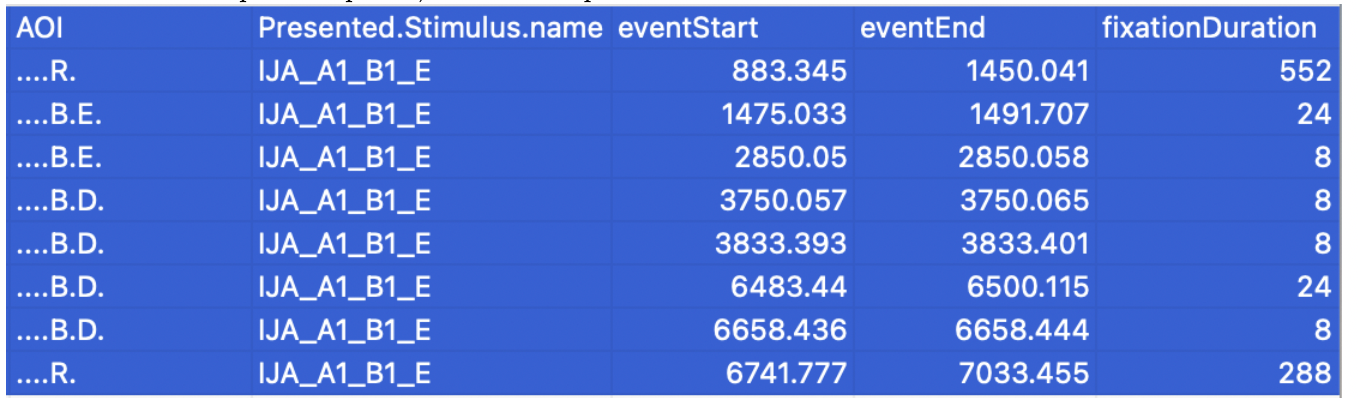
\includegraphics[scale=0.9]{"./dovalys.png"}}
\centering
\end{figure}

\begin{figure}[t]
\caption{Fixações Dovalys IJA.A1.B1.E.}
\noindent\makebox[\textwidth]{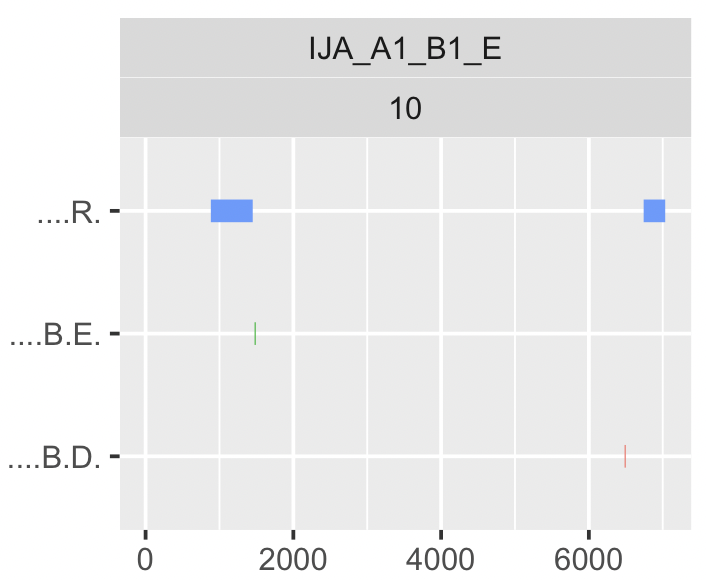
\includegraphics[scale=1]{"./dovalysgraph.png"}}
\centering
\end{figure}


\begin{figure}[t]
\caption{Abacaxi}
\noindent\makebox[\textwidth]{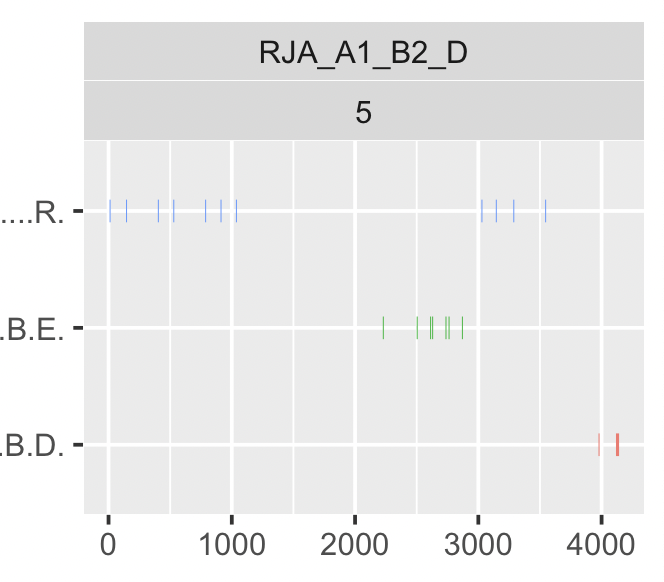
\includegraphics[scale=1]{"./abacaxi.png"}}
\centering
\end{figure}



\end{document}


